\documentclass[a4paper]{article}

%--------------------------------------------------------------------------
\usepackage[a4paper, total={6in, 9in}]{geometry}
\usepackage{amsmath}
\usepackage{booktabs}
\usepackage{caption}
\usepackage{graphicx}
\usepackage{float}
\usepackage{inconsolata}
\usepackage{listings}
\usepackage{siunitx}
\usepackage[most]{tcolorbox}
\usepackage{xfrac}
\usepackage{color}
\usepackage{setspace}
\usepackage{url}

%---------------------------------------------------------------------------

\lstdefinestyle{Python}{
	language        = Python,
	basicstyle      = \ttfamily,
	keywordstyle    = \color{blue},
	keywordstyle    = [2] \color{teal}, % just to check that it works
	stringstyle     = \color{green},
	commentstyle    = \color{red}\ttfamily
}

%--------------------------------------------------------------------------
\graphicspath{{./fig/}}

%--------------------------------------------------------------------------

\newtcblisting[auto counter]{sexylisting}[2][]{sharp corners, 
    fonttitle=\bfseries, colframe=gray, listing only, 
    listing options={basicstyle=\ttfamily,language=Python}, 
    title=Listing \thetcbcounter: #2, #1}

%--------------------------------------------------------------------------
\begin{document}

\title{Udacity: Search and Sample Return Report}
\author{Shane Reynolds}
\maketitle

\tableofcontents

\newpage

%--------------------------------------------------------------------------
\section{Introduction \& Background}
A simplistic and wide reaching definition of a robot is a machine which performs a task with some level of autonomy. In this context, robotic systems are appealing as they allow humans to avoid work that is considered dull, dirty and dangerous. This broad definition somewhat obfuscates the elements that make robotics work. Indeed, there is no clear consensus as to the mandatory sub-systems which comprise a robotic system, however, there are some common features which can be observed across many existing robotics platforms, these include:
\begin{itemize}
\item \textbf{Perception systems}: systems which allow the robot to perceive the world around it
\item \textbf{Decision making systems}: systems which allow the robot to decide a course of action given some information set
\item \textbf{Actuation systems}: systems which allow the robot to physically interact with the world
\end{itemize}

This project serves as a short introduction to these three systems. Principally, it touches on elementary image processing concepts, and very briefly explores some basic decision making. The project is based on a simulated mobile robot operating in a simple terrain environment. The simulation is built in Unity and the main python script which gives the robot perception and decision making capabilities is called \verb|perception.py| and \verb|decision.py|, respectively. Finally, the interface between image processing, decision making algorithms, and the simulation is driven by SocketIO. A screen shot of the simulation can be seen in Figure 1 below.

\vspace{1cm}

\begin{figure}[h]
\centering
\frame{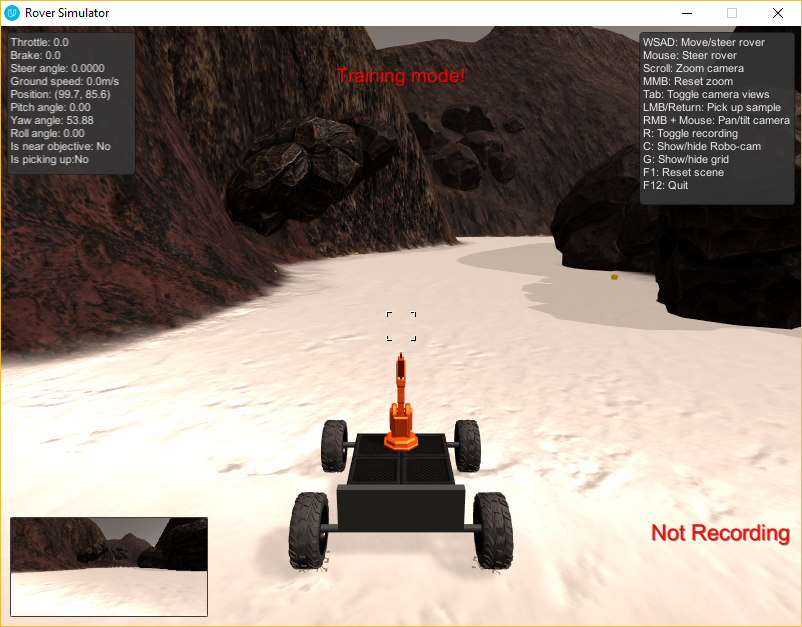
\includegraphics[scale=0.3]{image1}}
\caption{A screenshot of the mobile robotic rover at a standstill in the simulated environment.}
\end{figure}

\newpage

%--------------------------------------------------------------------------
\section{Methods and Implementation}
\subsection{Sensor Data}
The robot perceives its world via sensors. The main sensor used in this project is the camera mounted to the front of the robot. Figure 2 shows an example of a single image captured from the rover's camera. The camera images are received approximately once every 27$\si{\milli\second}$, or 36$\si{\hertz}$.

\begin{figure}[h]
\centering
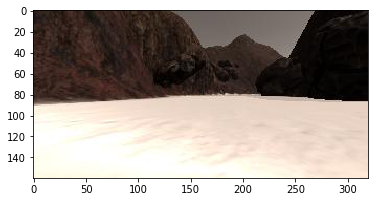
\includegraphics[scale=0.5]{image2}
\caption{A single image of the simulated environment as shown from the robot's front mounted camera.}
\end{figure}

In addition to the camera data, the there are sensors which measure the rover's position and orientation in space. Position is given by simple Cartesian coordinates, $(x, y)$, with reference to a fixed world frame. Orientation is given by roll, pitch, and yaw which are also with reference to the fixed world frame. Finally, throttle, brake, and steering angle of the rover are also provided. These values values are received at the same frequency as the images. The sensor data is used to help determine a course of action for the robot. This is achieved with two principal functions: \verb|perception_step| and \verb|decision_step|. Table 1 shows the different sensors data types, and a basic description of use of the captured data. 

\begin{table}[h]
\caption{A table which shows the different sensor data types, and their python format.}
\footnotesize
\begin{tabular}{llp{10cm}}
\toprule
\textbf{Sensor Data Type} & \textbf{Variable} & \textbf{Description}\\
\midrule
Image & \verb|img| & The image which is captured by the rover's front mounted camera - it is an \verb|np.array| of dimension $(160,320,3)$ and type \verb|uint8|\\
 & & \\
Position & \verb|pos| & Position of the rover with respect to a fixed world coordinate frame - it is a tuple of type \verb|np.float| \\
 & & \\
Yaw & \verb|yaw| & 	The yaw of the rover with respect to the world coordinate frame - it is of type \verb|np.float| and is one part of the rover orientation description\\
 & & \\
Pitch & \verb|pitch| & The pitch of the rover with respect to the world coordinate frame - it is of type \verb|np.float| and is one part of the rover orientation description\\
 & & \\
Roll & \verb|roll| & The roll of the rover with respect to the world coordinate frame - it is of type \verb|np.float| and is one part of the rover orientation description\\
 & & \\
Current Velocity & \verb|velocity| & The velocity of the rover - is of type \verb|np.float| and is capped at 2$\si{\meter\per\second}$ in this project\\
 & & \\
Steering Angle & \verb|steer| & The steering angle of the rover is determined by the angle of the front wheels with the centre line axis of the rover - is of type \verb|np.float| and is bound between $\pm 15 \si{\deg}$\\
 & & \\
Throttle Value & \verb|throttle| & Represents the value of locomotive force applied by the rover motors - is of type \verb|np.float| and is binary in opearation in that throttle is either applied, or not\\
 & & \\
Brake Value & \verb|brake| & Represents the applied force opposing motion (due to friction)\\
\bottomrule
\end{tabular}
\end{table}
\newpage
%--------------------------------------------------------------------------
\subsection{Image Processing}
Image processing represents a large component of the project, and consists of multiple stages. It is encapsulated in the \verb|perception_step| function, and is applied to each image captured by the rover's front mounted camera. The processing consists of three principal components: perspective transformation, segmentation, and translating the image to obtain a rover centric coordinate system. There is no fixed order in which the perspective transformation and segmentation steps need to occur, however, the transformation to a rover centric coordinate system can only be performed once the image has undergone a perspective transformation. The following subsections decribe each component in more detail.

%--------------------------------------------------------------------------
\subsubsection{Perspective Transformation}
To make navigation easier to comprehend for observers of the rover behaviour, it is often useful to implement a perspective transforms. Certainly, the rover is capable of navigating via the front mounted RGB camera, however, it is often useful to transform this view into a top down perspective. The process for implementing such a transform involves the following four steps:
\begin{enumerate}
\item Define four $(x,y)$ points in the source image (the image from the front mounted camera);
\item Identify the four $(x,y)$ points, defined from the source image, in the destination image (the top down image);
\item Using the information from steps 1) and 2), create a transformation matrix which will transform the points from the source image to the destination image;
\item Apply the transformation matrix to captured image arrays to convert the images from the front mounted camera to a top down perspective.
\end{enumerate}  

Often is it useful to apply a grid of known size to both the source and destination images to help with the identification of points in each image. The grid applied in this instance was a 1$\si{\meter}$ by 1$\si{\meter}$ grid, and can be seen in Figure 3. The points used in both the source image and destination image to build the transformation matrix can be seen in Table 2, and the code snippet showing the set-up of the parameters used for the perspective transformation can be seen in Listing 1. Finally, once the transformation matrix is determined, then it can be applied to each received image to transform the perspective from the front mounted camera to the top down view - a demonstration of this can be seen in Figure 5. It is worth noting that it should be expected that the perspective transform will have regions of black present in transformed image - these black areas represent the rover's blind spots. The perspective transform function can be seen in Listing 2.

\begin{figure}[h]
	\begin{minipage}[m]{0.45\linewidth}
		\centering
		\captionof{table}{The points determined from the destination and source images use to create the perspective transformation matrix.}
		\vspace{0.25cm}
		\begin{tabular}{ll}
		\toprule
		\textbf{Source} & \textbf{Destination}\\
		\midrule
		P1 & P1\\
		P1 & P1\\
		P1 & P1\\
		P1 & P1\\
		\bottomrule
		\end{tabular}
	\end{minipage}
	\hspace{0.5cm}
	\begin{minipage}[m]{0.45\linewidth}
		\centering
		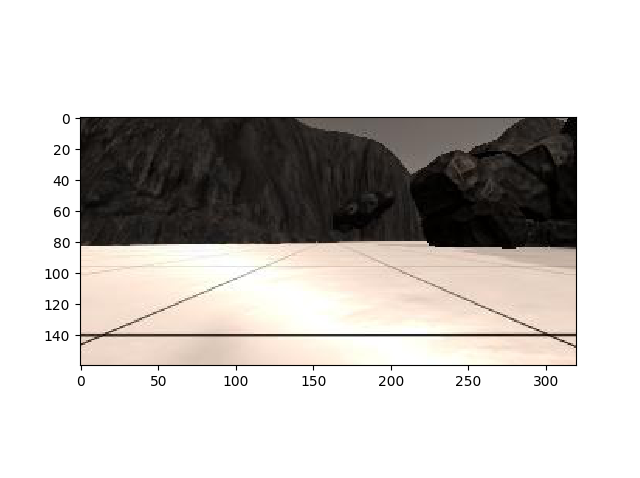
\includegraphics[scale=0.5]{image3}
		\vspace{-1cm}
		\caption{A 1x1 meter grid used to help establish points of reference.}
	\end{minipage}
\end{figure}

\begin{figure}[h]\scriptsize
\begin{sexylisting}{Set up of the parameters which are used for the perspective transform.}
img = Rover.img # takes the current camera image from the Rover and stores it in img
dst_size = 5 # what does this do
bottom_offset = 6 # what does this do
		
# Create the source array 
source = np.float32([[14, 140], [301 ,140],[200, 96], [118, 96]]) # specify the source array
destination = np.float32([[img.shape[1]/2 - dst_size, img.shape[0] - bottom_offset],
	                  [img.shape[1]/2 + dst_size, img.shape[0] - bottom_offset],
			  [img.shape[1]/2 + dst_size, img.shape[0] - 2*dst_size - bottom_offset], 
			  [img.shape[1]/2 - dst_size, img.shape[0] - 2*dst_size - bottom_offset],
			  ])	
\end{sexylisting}
\end{figure}

\begin{figure}[h]\scriptsize
\begin{sexylisting}{Code for the perspective transform function implementation.}
def perspect_transform(img, src, dst):
           
    M = cv2.getPerspectiveTransform(src, dst)
    
    # Keep same size as input image
    warped = cv2.warpPerspective(img, M, (img.shape[1],img.shape[0]))
    
    return warped
\end{sexylisting}
\end{figure}

\begin{figure}[H]
	\centering
	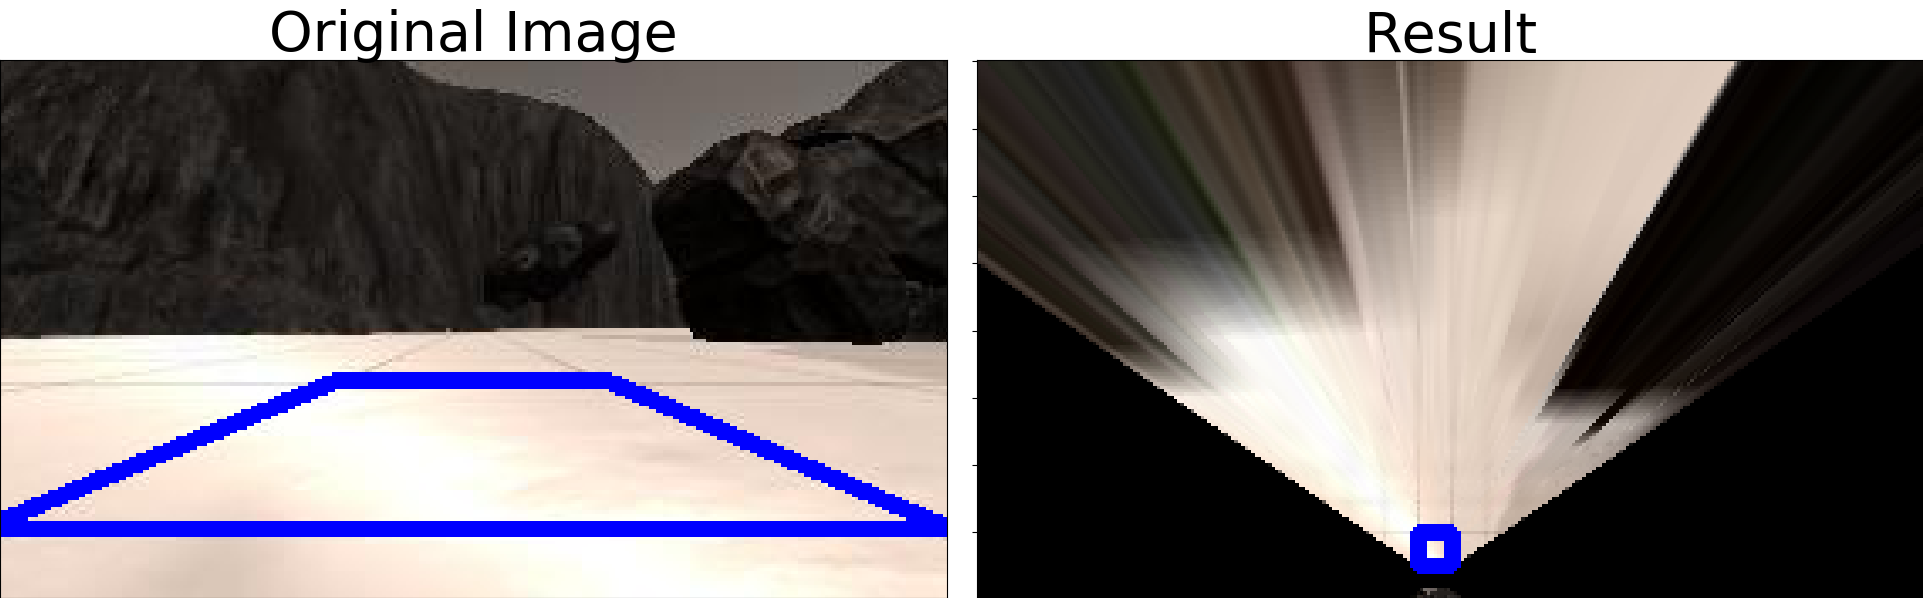
\includegraphics[scale=0.3]{image4}
	\caption{The original image from the rover's front mounted camera can be seen on the left, with the image after the perspective transform has been applied can be seen on the right.}
\end{figure}

\subsubsection{Segmentation: Navigable Terrain \& Obstacles}
There are 3 different types of object that are of interest to the rover: navigable terrain, obstacles, and rock samples. A simple way to obtain the navigable terrain is to create a basic RGB filter. This works because it exploits the stark contrast between obstacles (which are dark), and navigable terrain (which is light). It must be noted that this technique would not generalise well, and would obviously perform best in environments with similar features to the simulation. Looking more closely at the filter, we see that we are able to extract both navigable terrain and obstacles with one instance of filtering since these two types of terrain are mutually exclusive - to put this simply: if the terrain is not navigable, then it must be an obstacle. The filtering itself is simplistic in its implementation, using an upper threshold for each of the R, G, and B values. To determine the cut-off threshold for each of the R, G, and B channels, most Operating Systems come with a basic image viewer which will provide information for each of the R, G, and B channels by pixel. A single frame of navigable terrain was loaded into an image viewer. Using this crude analysis values of 160 for each of the R, G, and B channels were determined as an appropriate threshold for navigable terrain. This process can be seen in Figure 5.

\begin{figure}[h]
	\centering
	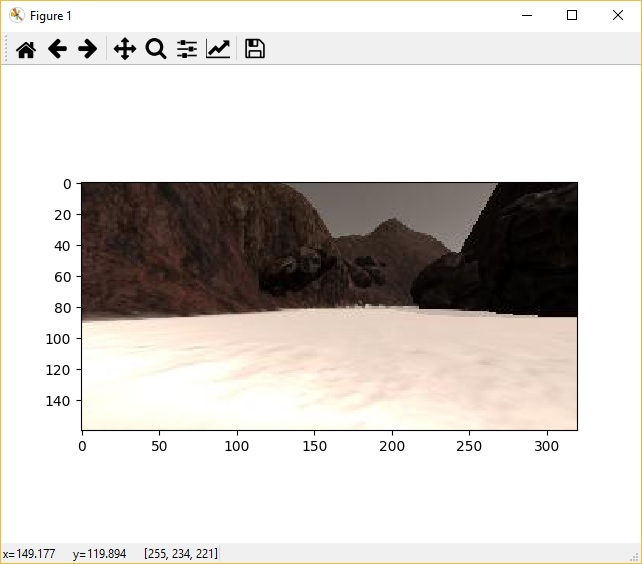
\includegraphics[scale=0.4]{rock_test}
	\caption{Using XXXX a crude analysis of the image was undertaken to determine the threshold values for R, G, and B values which represent navigable terrain.}
\end{figure}

Implementation of the colour threshold function can be seen in Listing 3. If a pixel in an image has R, G, and B values which are all greater than 160, the pixel is classified as navigable terrain. An example of the classification of navigable terrain can be seen in Figures 6 and 7.

\vspace{0.5cm}

\begin{figure}[H]\scriptsize
\begin{sexylisting}{Insert caption}
def color_thresh(img, rgb_thresh=(160, 160, 160)):
    # Create an array of zeros same xy size as img, but single channel
    color_select = np.zeros_like(img[:,:,0])
    # Require that each pixel be above all three threshold values in RGB
    # above_thresh will now contain a boolean array with "True"
    # where threshold was met
    above_thresh = (img[:,:,0] > rgb_thresh[0]) \
                & (img[:,:,1] > rgb_thresh[1]) \
                & (img[:,:,2] > rgb_thresh[2])
    # Index the array of zeros with the boolean array and set to 1
    color_select[above_thresh] = 1
    # Return the binary image
    return color_select
\end{sexylisting}
\end{figure}

\vspace{0.5cm}

\begin{figure}[h]
\centering
	\begin{minipage}[t]{0.45\linewidth}
	\centering
	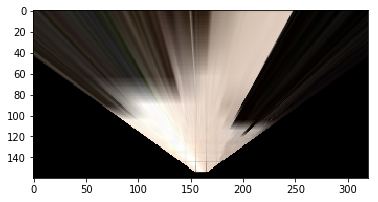
\includegraphics[scale=0.5]{image6}
	\caption{The perspective transformed image prior to the segmentation filter application.}
	\end{minipage}
	\hspace{0.5cm}
	\begin{minipage}[t]{0.45\linewidth}
	\centering
	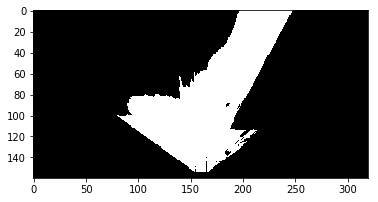
\includegraphics[scale=0.5]{image7}
	\caption{The perspective transformed image after the segmentation filter is applied - note that this is shown in grayscale.}
	\end{minipage}
\end{figure}

\newpage

Whilst this method can be applied successfully to determine navigable terrain, incorrect results maybe obtained when segmenting obstacles. This is caused if the filter is applied without consideration of the rover's blind spot, which is the area behind the rover's camera. In order to account for the rover's blind spot the segmentation filter needs to be applied prior to the perspective transform. This allows the capture of a conical region where the rover cannot see. This additional information, used in conjunction with a binary inverse of the navigable terrain array, provides for higher levels of accuracy when segmenting obstacles - implementation of this can be seen in Listing 4. The listing shows the extraction of the \verb|cone| array, and the \verb|rock| array (which is covered in the following sub-section) and finally subtracts them from the \verb|obstacle_temp| array to obtain the \verb|obstacle| array.\\

An example of the full process for extracting navigable terrain and obstacles can be seen in Figures 8, 9, 10, 11, 12 and 13. The first figure in the sequence shows the image from the camera on the front of the rover, and Figure 9 shows the perspective transform. Figure 10 shows the navigable terrain after the segmentation filer is applied using a threshold value of 165 for R, G, and B channels. Figure 11 and 12 show the navigable terrain inverse, and the cone, respectively. Finally, Figure 13 shows the obstacles. Figures 10 and 13 are combined to provide a full map which shows navigable terrain in blue and obstacles in red. It must be noted that applying segmentation filters prior to perspective transforms is desirable since the code implementations would be simplified, however, in practice this structure degrades the quality overall segmentation resulting in poorer performance.\\

\vspace{1cm}

\begin{figure}[h]\scriptsize
\begin{sexylisting}{test}
# Apply perspective transform
warped = perspect_transform(img, source, destination)
    
# Apply color threshold to identify navigable terrain/obstacles/rock samples
# Threshold image for terrain
nav = color_thresh(warped, (165, 165, 165))
    
# Threshold image for gold rocks
hsv_warped = cv2.cvtColor(warped, cv2.COLOR_RGB2HSV)
lower_thres = np.array([0,100,110])
upper_thres = np.array([70,255,255])
rock = cv2.inRange(hsv_warped, lower_thres, upper_thres).astype(bool).astype(int)
    
# Threshold image for obstacles
obstacles_temp = color_thresh(warped, (135, 135, 135))
obstacles_temp ^= 1
    
# Threshold image for cone
# Cone derivation
nav_thresh = color_thresh(img, (165, 165, 165))
obstacles_thresh = nav_thresh.copy()
obstacles_thresh ^= 1
cone = perspect_transform(obstacles_thresh, source, destination)
cone ^= 1
cone = np.logical_and(obstacles_temp, cone)
    
# Thresholded image for obstacles (with cone and rocks removed)
obstacles = obstacles_temp - cone - rock
\end{sexylisting}
\end{figure}

\begin{figure}[h]
	\centering
	\begin{minipage}[t]{0.45\linewidth}
	\centering
	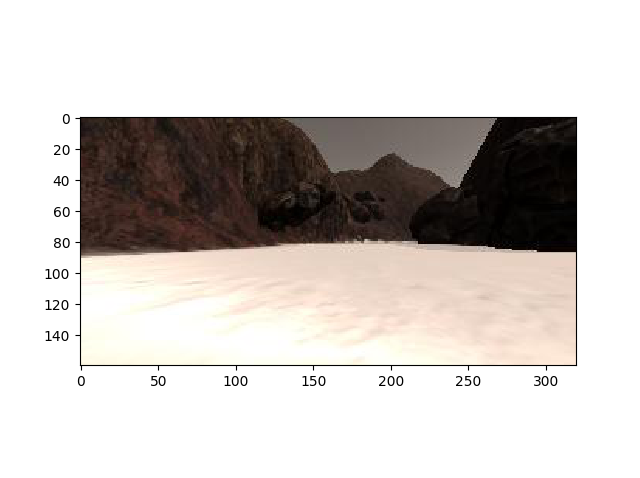
\includegraphics[scale=0.45]{image8}
	\vspace{-1.5cm}
	\caption{The original image taken from the camera mounted to the front of the rover.}
	\end{minipage}
	\hspace{0.5cm}
	\begin{minipage}[t]{0.45\linewidth}
	\centering
	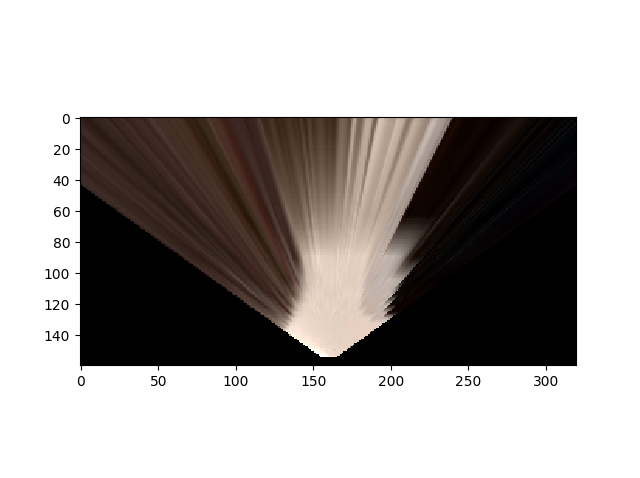
\includegraphics[scale=0.45]{image9}
	\vspace{-1.5cm}
	\caption{The image once it has undergone the perspective transform discussed in Section 2.2.1.}
	\end{minipage}
\end{figure}

\begin{figure}[h]
	\centering
	\begin{minipage}[t]{0.45\linewidth}
	\centering
	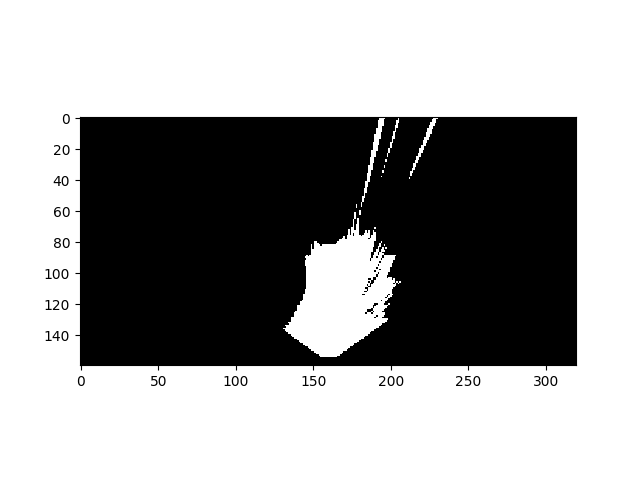
\includegraphics[scale=0.45]{image10}
	\vspace{-1.5cm}
	\caption{The resultant image of the segmentation for navigable terrain. Note that the white areas depict the navigable terrain areas.}
	\end{minipage}
	\hspace{0.5cm}
	\begin{minipage}[t]{0.45\linewidth}
	\centering
	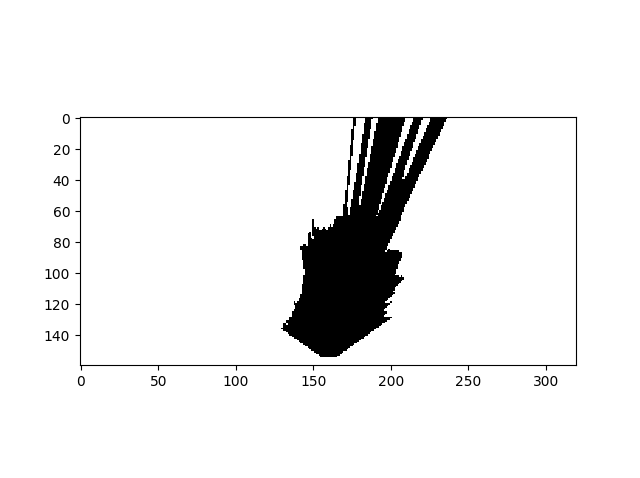
\includegraphics[scale=0.45]{image11}
	\vspace{-1.5cm}
	\caption{The resultant image for the inverse of the navigable terrain.}
	\end{minipage}
\end{figure}

\begin{figure}[h]
	\centering
	\begin{minipage}[t]{0.45\linewidth}
	\centering
	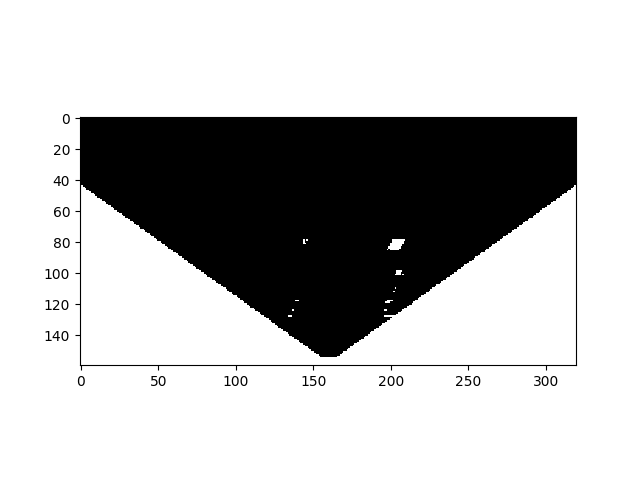
\includegraphics[scale=0.45]{image12}
	\vspace{-1.5cm}
	\caption{The resultant image for the derivation of rover blind spot.}
	\end{minipage}
	\hspace{0.5cm}
	\begin{minipage}[t]{0.45\linewidth}
	\centering
	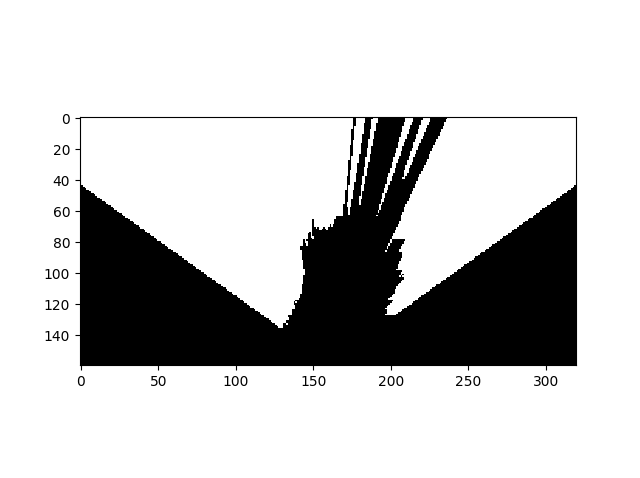
\includegraphics[scale=0.45]{image13}
	\vspace{-1.5cm}
	\caption{The final image which shows the rover obstacles. Note that the white areas depict the rover obstacles.}
	\end{minipage}
\end{figure}

\clearpage

\subsubsection{Segmentaiton: Rock Samples}

Providing segmentation for rock samples saw unstable performance when filtering using RGB channels. This is due to the sample rocks holding different RGB values in darker regions, when compared to samples in lighter regions. Put simply, shadows affect the segmentation performance. An alternative colour representation known as Hue, Saturation, Value (HSV) is less susceptible to performance degradation from shadows and was employed in this instance. To determine the HSV values for the sample, a method was employed similar to that seen in Figure 5. Figures 14, and 15 show the process of segmenting the rock samples. Figure 16 shows the completed perspective transformed and segmented image of the navigable terrain, obstacles, and rocks.

\vspace{1cm}

\begin{figure}[h]\scriptsize
\centering
\begin{sexylisting}{text}
# Apply perspective transform
warped = perspect_transform(img, source, destination)

# Threshold image for gold rocks
hsv_warped = cv2.cvtColor(warped, cv2.COLOR_RGB2HSV)
lower_thres = np.array([0,100,110])
upper_thres = np.array([70,255,255])
rock = cv2.inRange(hsv_warped, lower_thres, upper_thres).astype(bool).astype(int)
\end{sexylisting}
\end{figure}

\vspace{-0.5cm}

\begin{figure}[h]
\centering
\begin{minipage}[t]{0.45\linewidth}
\centering
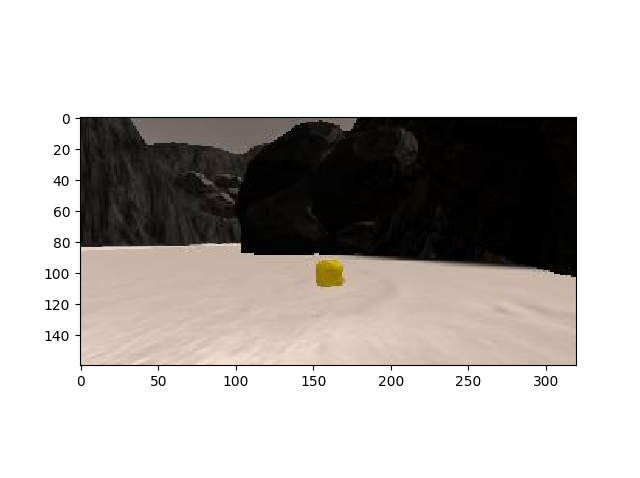
\includegraphics[scale=0.45]{image15}
\vspace{-1.5cm}
\caption{include a graphic of the original rock image}
\end{minipage}
\hspace{0.5cm}
\begin{minipage}[t]{0.45\linewidth}
\centering
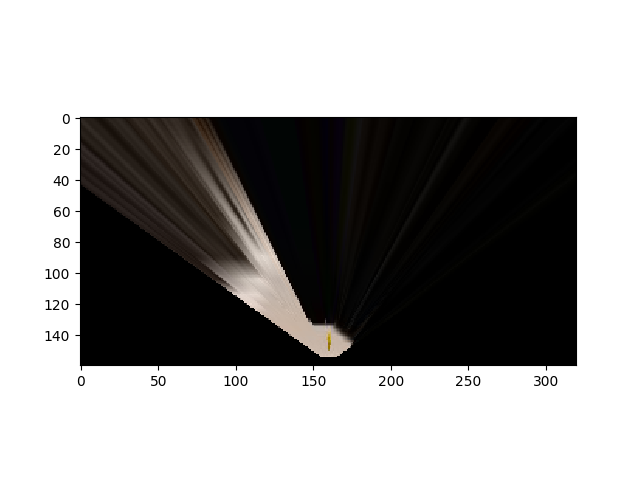
\includegraphics[scale=0.45]{image16}
\vspace{-1.5cm}
\caption{include a graphic of the filtered image - gray scale}
\end{minipage}
\end{figure}

\vspace{-1cm}

\begin{figure}[h]
\centering
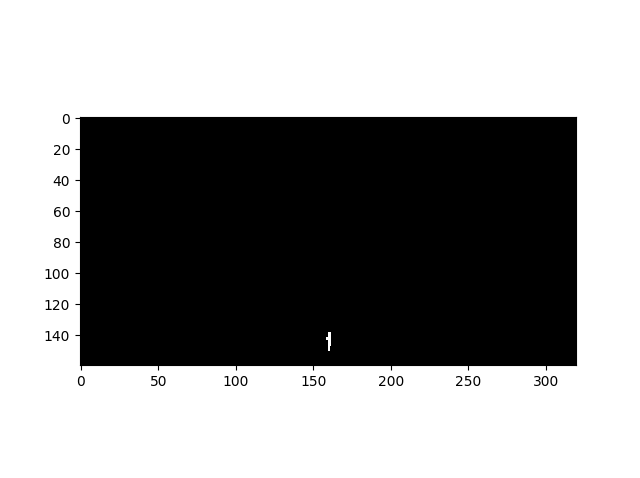
\includegraphics[scale=0.55]{image17}
\vspace{-1cm}
\caption{Include an image of the full image transformation with the rock and the blue and green}
\end{figure}

\newpage

\subsubsection{Rover Centric Coordinates}
A coordinate frame is attached to the rover, in addition to establishing a fixed world coordinate frame. Assigning coordinate frames in this way allows the mathematical description of both position and orientation of the rover with respect to the world. A pictorial representation of the coordinate assignment can be seen in Figure 17.\\

\vspace{1cm}

\begin{figure}[h]
\centering
\frame{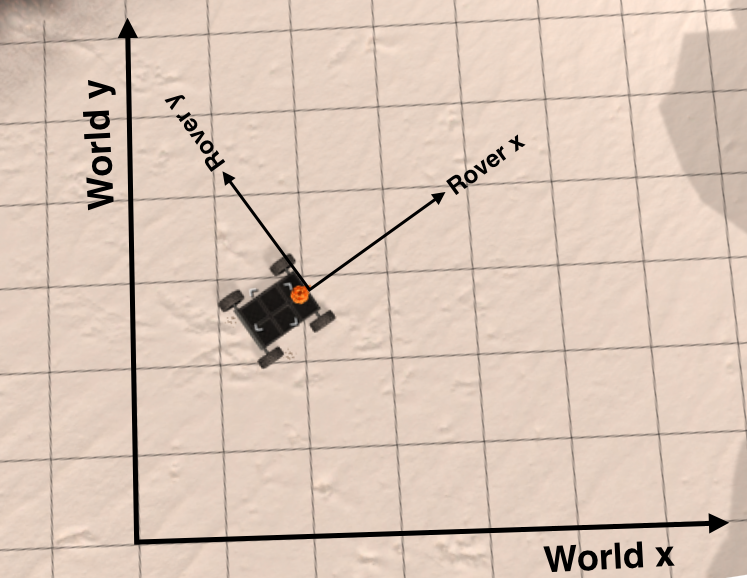
\includegraphics[scale=0.3]{image14}}
\caption{A coordinate frame is attached to, and moves with, the rover. This rover coordinate frame exists in the fixed world frame.}
\end{figure}

\vspace{1cm}

The image that is captured and processed by the \verb|XXXX| function uses the source and destination points to map the recieved image into a 2D top down view point. Unfortunately, this function does not provide the correct orientation of the image with respect to the rover coordinate frame - this is shown in Figure 18. To ensure that the image is correctly positioned and oriented a coordinate frame transformation is performed, called \verb|XXXX|, shown in Listing 6. This transformation translates the image so that it is positioned along the $x$-axis of the coordinate frame, and flips the $x$ and $y$ axes. The image which has been correctly positioned on the rover coordinate frame can be seen in Figure 19. 

\vspace{1cm}

\begin{figure}[h]\scriptsize
\centering
\begin{sexylisting}{text}
def rover_coords(binary_img):
    # Identify nonzero pixels
    ypos, xpos = binary_img.nonzero()
    # Calculate pixel positions with reference to the rover position being at the 
    # center bottom of the image.  
    x_pixel = -(ypos - binary_img.shape[0]).astype(np.float)
    y_pixel = -(xpos - binary_img.shape[1]/2 ).astype(np.float)
    return x_pixel, y_pixel
\end{sexylisting}
\end{figure}

\vspace{2cm}

\begin{figure}[h]
\centering
\begin{minipage}[t]{0.45\linewidth}
\centering
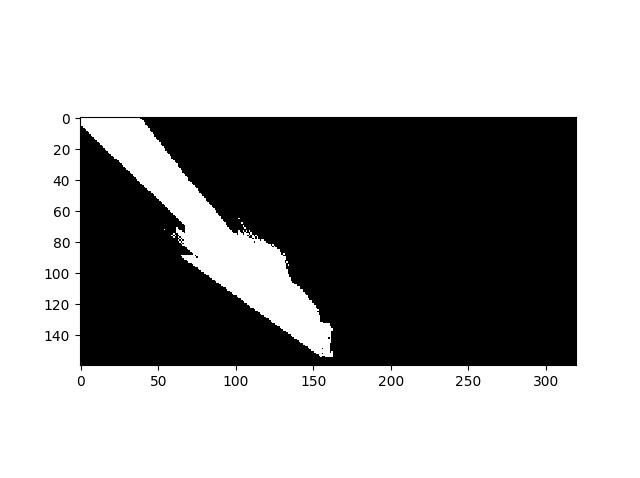
\includegraphics[scale=0.45]{image19}
\caption{include a non-transformed image}
\end{minipage}
\hspace{0.5cm}
\begin{minipage}[t]{0.45\linewidth}
\centering
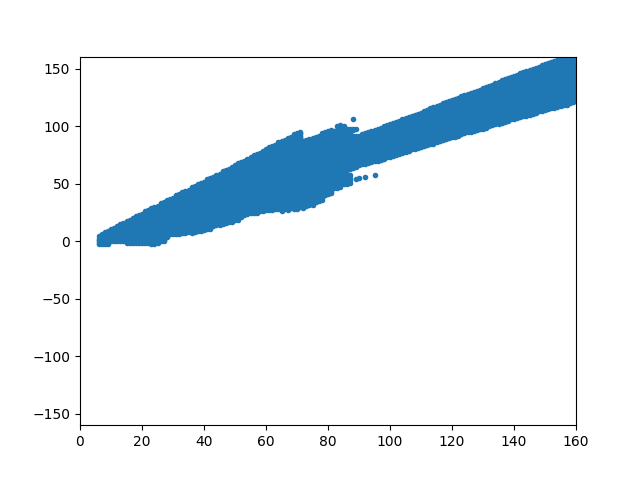
\includegraphics[scale=0.45]{image20}
\caption{include an image of the transformed rover centric coord system}
\end{minipage}
\end{figure}

\subsubsection{Mapping the the World Coordinate Frame}

The rover navigates around the simulated environment generating information about the environment topology, using the segmentation techniques described in sections 2.2.2 and 2.2.3. Essentially, the rover captures information on navigable terrain and obstacles, and creates a map of the world. In order to do this, image information being processed needs to be transformed from the rover coordinate frame to the world coordinate frame. This requires further transformation. Listings 7, and 8 provide a function for 2D rotation, and 2D translation, respectively. Listing 9 uses both Listings 7, and 8 to perform the full transformation from rover to world coordinate frame. Figure 20 provides an example of the map that generated by the rover.

\vspace{1cm}

\begin{figure}[h]\scriptsize
\begin{sexylisting}{insert text}
# A function which provides rotation in 2D
def rotate_pix(xpix, ypix, yaw):
    # Convert yaw to radians
    yaw_rad = yaw * np.pi / 180
    xpix_rotated = (xpix * np.cos(yaw_rad)) - (ypix * np.sin(yaw_rad))
                            
    ypix_rotated = (xpix * np.sin(yaw_rad)) + (ypix * np.cos(yaw_rad))
    # Return the result  
    return xpix_rotated, ypix_rotated
\end{sexylisting}
\end{figure}

\begin{figure}[h]\scriptsize
\begin{sexylisting}{insert text}
# A functions which provides a translation in 2D
def translate_pix(xpix_rot, ypix_rot, xpos, ypos, scale): 
    # Apply a scaling and a translation
    xpix_translated = (xpix_rot / scale) + xpos
    ypix_translated = (ypix_rot / scale) + ypos
    # Return the result  
    return xpix_translated, ypix_translated
\end{sexylisting}
\end{figure}

\begin{figure}[h]\scriptsize
\begin{sexylisting}{insert text}
# A function which performs the transformation from rover to world coordinates
def pix_to_world(xpix, ypix, xpos, ypos, yaw, world_size, scale):
    # Apply rotation
    xpix_rot, ypix_rot = rotate_pix(xpix, ypix, yaw)
    # Apply translation
    xpix_tran, ypix_tran = translate_pix(xpix_rot, ypix_rot, xpos, ypos, scale)
    # Perform rotation, translation and clipping all at once
    x_pix_world = np.clip(np.int_(xpix_tran), 0, world_size - 1)
    y_pix_world = np.clip(np.int_(ypix_tran), 0, world_size - 1)
    # Return the result
    return x_pix_world, y_pix_world
\end{sexylisting}
\end{figure}

\begin{figure}[h]
\centering

\includegraphics[scale=0.5]{placeholder}
\caption{Show a picture of the mapped terrain, if possible}
\end{figure}

\newpage

%--------------------------------------------------------------------------
\subsection{Autonomous Navigation}
The rover is designed to move about the simulated environment autonomously. The main code executing the autonomous mode of navigation is encapsulated in \verb|drive_rover.py|, shown in Appendix B. There are two key functions which are executed in this script: \verb|perception.py| and \verb|decision.py|. The \verb|perception.py| function processes rover captured images, and provides an information set which is used by the \verb|decision.py| function as input for autonomous navigation. Each of the functions are discussed in more detail below.

\subsubsection{Perception Step}
The perception step is applied to each image that is captured by the rover's front mounted camera. As previously mentioned, images are captured at approximately 36 $\si{\hertz}$. The \verb|perception_step| function can be seen, in full, in Appendix A. The function takes a single object oriented arguement, which details the current state of the rover, including the latest image captured by the camera. Using the image, navigable terrain, obstacles, and the prescence of rocks are determined and updated on the world map. Listing 10 shows the code which provides for world map updating - obstacles are on the red channel, navigable terrain is on the blue channel, and rocks are on the green channel.

\begin{figure}[h]\scriptsize
\begin{sexylisting}{insert text}
# Add a small amount of colour to obstacles
    Rover.worldmap[obstacle_y_world, obstacle_x_world, 0] += 2
    # Reset obstacle channel that rover currently sees as navigable terrain
    Rover.worldmap[nav_y_world, nav_x_world, 0] = 0
    
    # Update any rocks on the rock colour channel
    Rover.worldmap[rock_y_world, rock_x_world, 1] = 255 
    
    # Reset anything on the navigable terrain channel that the rover currently sees as an obstacle
    Rover.worldmap[obstacle_y_world, obstacle_x_world, 2] = 0
    Rover.worldmap[nav_y_world, nav_x_world, 2] = 255
\end{sexylisting}
\end{figure}

It is important to note that the segmentation of navigable terrain, and obstacles, in the current image can be in conflict with historically recorded areas on the world map. To put this simply, the segmentation of obstacles and navigable terrain is imperfect - this leads to differing results in images of the same area. To overcome this, when the red channel (obstacles) is being updated, all navigable terrain pixels in the current image are set to zero. Similarly, when the blue channel is being updated, all obstacles pixels in the current image are set to zero. This ensures that pixels in the world map are never simultaneously an obstacle and navigable terrain.

The main importance of the perception step is to take an image an to organise it into meaningful information so that decisions can be made using the decision step. Important parts are:
\begin{itemize}
\item determining the navigation angle based on the navagble terrain available
\item determining if a rock can be seen, and switching the rover mode into one which readys the rover for rock collection
\end{itemize}

The perception step also helps to determine whether there is a rock present in the image, and if so will direct the rover into rocking mode which collects rocks.

\begin{figure}[h]\scriptsize
\begin{sexylisting}
if (sum(sum(rock)) > 20) and Rover.mode != "stuck":
        Rover.mode = "rocking"
        Rover.rock_spot_count = 0 # The rover will reset the rock spot counter
        distances, angles = to_polar_coords(xpix_rock, ypix_rock)
        Rover.rock_dists = distances
        Rover.rock_angles = angles
    # If the Rover loses track of the rock, the Rover still remains in the rocking
    # mode, however, will start to count down to switching back to forward mode
    # provided the Rover cannot relocate the rock
    elif Rover.mode == "rocking":
        Rover.rock_spot_count += 1
        Rover.rock_angles = 0
\end{sexylisting}
\end{figure}

All navigation is done by taking navigation pixels determined by the segmentation function and converting them into angles using the polar conversion function

\begin{figure}[h]\scriptsize
\begin{sexylisting}{text}
def to_polar_coords(x_pixel, y_pixel):
    # Convert (x_pixel, y_pixel) to (distance, angle) 
    # in polar coordinates in rover space
    # Calculate distance to each pixel
    dist = np.sqrt(x_pixel**2 + y_pixel**2)
    # Calculate angle away from vertical for each pixel
    angles = np.arctan2(y_pixel, x_pixel)
    return dist, angles
\end{sexylisting}
\end{figure}

\subsubsection{Decision Step}
The \verb|decision.py| function, shown in Appendix C, is applied after the current image has been processed, and the rover state updated. Principally, this function is concerned with rover navigation and focuses on obstacles avoidance, in addition to providing the rover with some capacity to negotiate dead ends in the environment and locate rocks. The decision step decides between 4 distinct Rover modes: forward, rocking, stop, and stuck.\\

The forward state code snippet is shown in Listing 11, and the flow diagram explaining the logic behind the operation is shown in Figure 21. When in the forward state the rover checks that there is navigable terrain in front of it. If there is sufficient navigable terrain, and the velocity is at the maximum velocity, then the rover will continue in this mode. If the rover is below maximum velocity, then the throttle will be applied. If the rover has zero velocity, but has sufficient navigable terrain, then the clock for determining if the rover is stuck will start to count. If the stuck counter, which is stored in the object variable \verb|Rover.vel|, reaches 400, then the rover will change state from \verb|forward| to \verb|stuck|. The timer for this state change was implemented to provide some hysteresis preventing the rover from rapid state switching. Note that if the Rover's velocity reaches above a threshold while the stuck counter is counting, then it is deemed that the rover has freed itself from the obstacle and the counter is reset.\\

The steering direction is determined by a weighted moving average of the present steering angle stored in \verb|Rover.nav_angles|, with a weight of $\sfrac{1}{3}$, and the previous steering angle, with a weight of $\sfrac{2}{3}$. This provides a slight reduction in erratic corrections given extreme values in \verb|Rover.nav_angles|. Erratic changes are further ameliorated by bounding the steering angle between -15$^o$ and 15$^o$.

\vspace{2cm}

\begin{figure}[h]\scriptsize
\begin{sexylisting}{Code snippet for the operation of the forward state of the rover}
# Check for Rover.mode status
        if Rover.mode == 'forward':
            # If the Rover is no longer stuck, then 
            if abs(Rover.vel) > 0.08:
                Rover.vel_count = 0 # Reset the stuck counter
            # Check the extent of navigable terrain
            if len(Rover.nav_angles) >= Rover.stop_forward:  
                # If mode is forward, navigable terrain looks good 
                # and velocity is below max, then throttle 
                if Rover.vel < Rover.max_vel:
                    # Set throttle value to throttle setting
                    Rover.throttle = Rover.throttle_set
                    # If the rover is stuck
                    if abs(Rover.vel) < 0.05:
                        # Some hysteresis so the robot doesn't switch modes rapidly
                        Rover.vel_count += 1
                        if Rover.vel_count > 400:
                            Rover.vel_count = 0 # Reset the zero velocity count
                            Rover.stuck_count = 0 # Start the stuck counter
                            Rover.throttle = 0
                            Rover.brake = 0
                            Rover.steer = 0
                            Rover.mode = 'stuck'
                else: # Else coast
                    Rover.throttle = 0
                Rover.brake = 0
                
                # Set steering to average angle clipped to the range +/- 15
                # Note that the steering angle has been smoothed by using a
                # two time period weighted average
                Rover.steer =
	                (2*Rover.steer +
		                 np.clip(np.mean(Rover.nav_angles * 180/np.pi), -15, 15))/3
                
            # If there's a lack of navigable terrain pixels then go to 'stop' mode
            elif len(Rover.nav_angles) < Rover.stop_forward:
                    # Set mode to "stop" and hit the brakes!
                    Rover.throttle = 0
                    # Set brake to stored brake value
                    Rover.brake = Rover.brake_set
                    Rover.steer = 0
                    Rover.mode = 'stop'
\end{sexylisting}
\end{figure}

\newpage

\begin{figure}[h]
\hspace{-1.5cm}
\vspace{4cm}
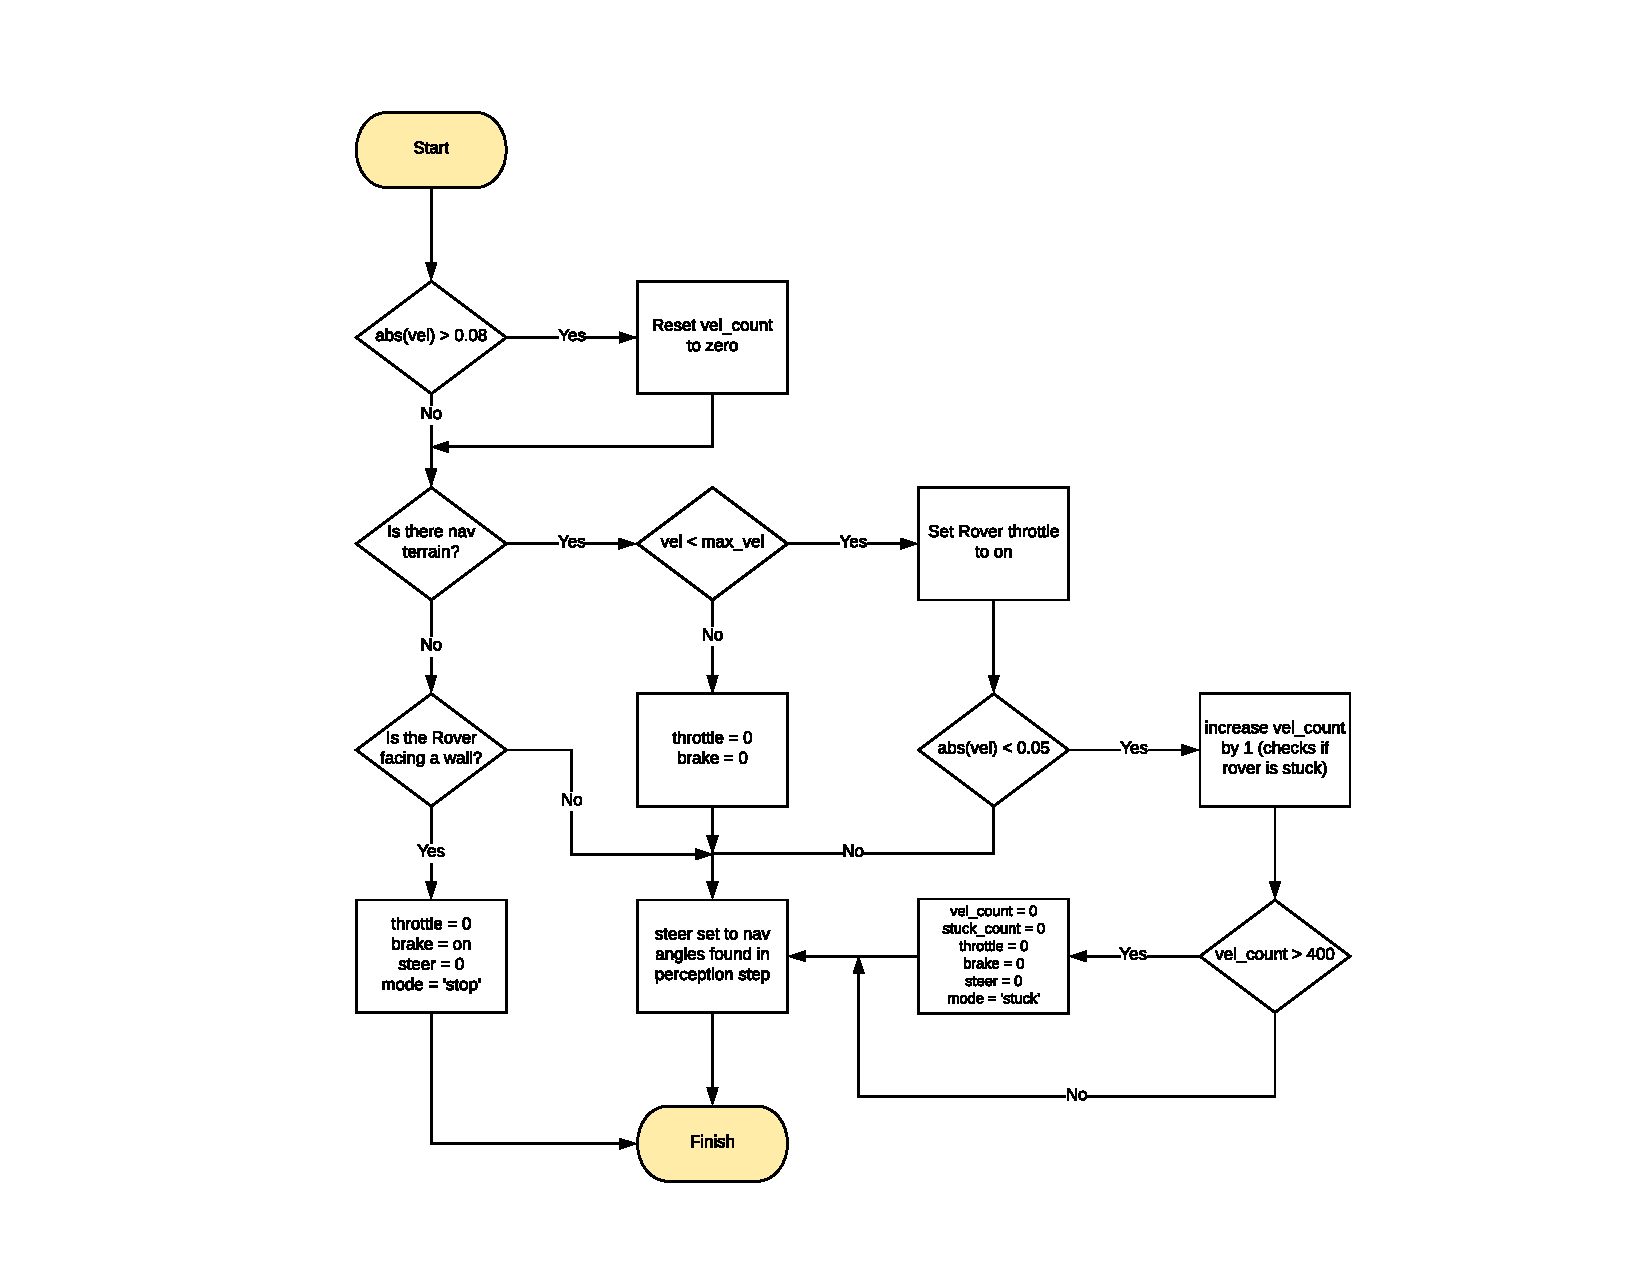
\includegraphics[scale = 0.7]{forward_flow}
\vspace{-3cm}
\caption{Flow diagram showing the operation of the rover when it is in the forward state of operation.}
\end{figure}

\newpage

The rocking state is used when the rover detects a rock, or the current image has rock like characteristics. The change from the current state to the rocking state is determined by the code snippet shown in Listing 12. This state change will occur if the rover is not in the stuck state, and there are more than 20 pixels in the current image which have the characteristics of a rock. Note that if the rover is in rocking mode, but loses track of the rock (that is the rock is not persistent in teh image) then a counter starts which will eventually switch the rover back to the forward state. The timer is employed to stop rapid state switching. The rocking state code snippet is shown in Listing 12, and the flow diagram explaining the logic behind the operation is shown in Figure 22.\\

\begin{figure}[h]\scriptsize
\begin{sexylisting}{Code snippet showing how the rover changes to the rocking state}
# If the rover detects a rock, and it is not in stuck mode, the Rover will
# switch to the rocking mode (i.e. the mode used to search for rocks)
if (sum(sum(rock)) > 20) and Rover.mode != "stuck":
	Rover.mode = "rocking"
	Rover.rock_spot_count = 0 # The rover will reset the rock spot counter
	distances, angles = to_polar_coords(xpix_rock, ypix_rock)
	Rover.rock_dists = distances
	Rover.rock_angles = angles
# If the Rover loses track of the rock, the Rover still remains in the rocking
# mode, however, will start to count down to switching back to forward mode
# provided the Rover cannot relocate the rock
elif Rover.mode == "rocking":
	Rover.rock_spot_count += 1
	Rover.rock_angles = 0
\end{sexylisting}
\end{figure}

\begin{figure}[h]\scriptsize
\begin{sexylisting}{Code snippet showing rover operation in the rocking state}
# If the rover is in the vicinity of a rock - this is set in perception 
        elif Rover.mode == 'rocking':
            if abs(Rover.vel) > 0.08:
                Rover.vel_count = 0 # Reset the stuck counter
            if Rover.rock_spot_count > 200:
                Rover.mode = "forward"
            else:
                if Rover.vel < 0.5:
                    Rover.throttle = 0.1
                    Rover.brake = 0
                    if abs(Rover.vel) < 0.05:
                        # Some hysteresis so the robot doesn't switch modes rapidly
                        Rover.vel_count += 1
                        if Rover.vel_count > 400:
                            Rover.vel_count = 0 # Reset the zero velocity count
                            Rover.stuck_count = 0 # Start the stuck counter
                            Rover.throttle = 0
                            Rover.brake = 0
                            Rover.steer = 0
                            Rover.mode = 'stuck'
                elif Rover.vel >= 0.5:
                    Rover.throttle = 0
                
                # This will direct the rover towards the rock
                Rover.steer = np.clip(np.mean(Rover.rock_angles * 180/np.pi), -15, 15)
                
                # This will stop the Rover if it is near a rock sample
                # Note this is a condition for picking up samples
                if Rover.near_sample:
                    Rover.throttle = 0
                    Rover.brake = Rover.brake_set
\end{sexylisting}
\end{figure}

When in the rocking state, the rover will first check if timer if the rock image has been lost. If the timer is greater than 200, then the rover will switch back to the forward state. The rover will then check if it is moving, and start a stuck counter similar to that used in forward mode if the velocity is below a certain threshold. If the counter \verb|Rover.vel_count| goes above 400 then the rover will switch to the stuck state. Provided the rover remains in the rocking state, the rover will approach the rock using \verb|Rover.rock_angles| to steer, at a maximum velocity of 0.5. Note that if the rover loses track of the rock image, then the steering angle is set to 0. Once the rover is near the sample, the \verb|Rover.near_sample| flag is tripped, and the rover will stop to pick up the rock, after which the state will change to forward.\\

\begin{figure}[h]
\hspace{-2.5cm}
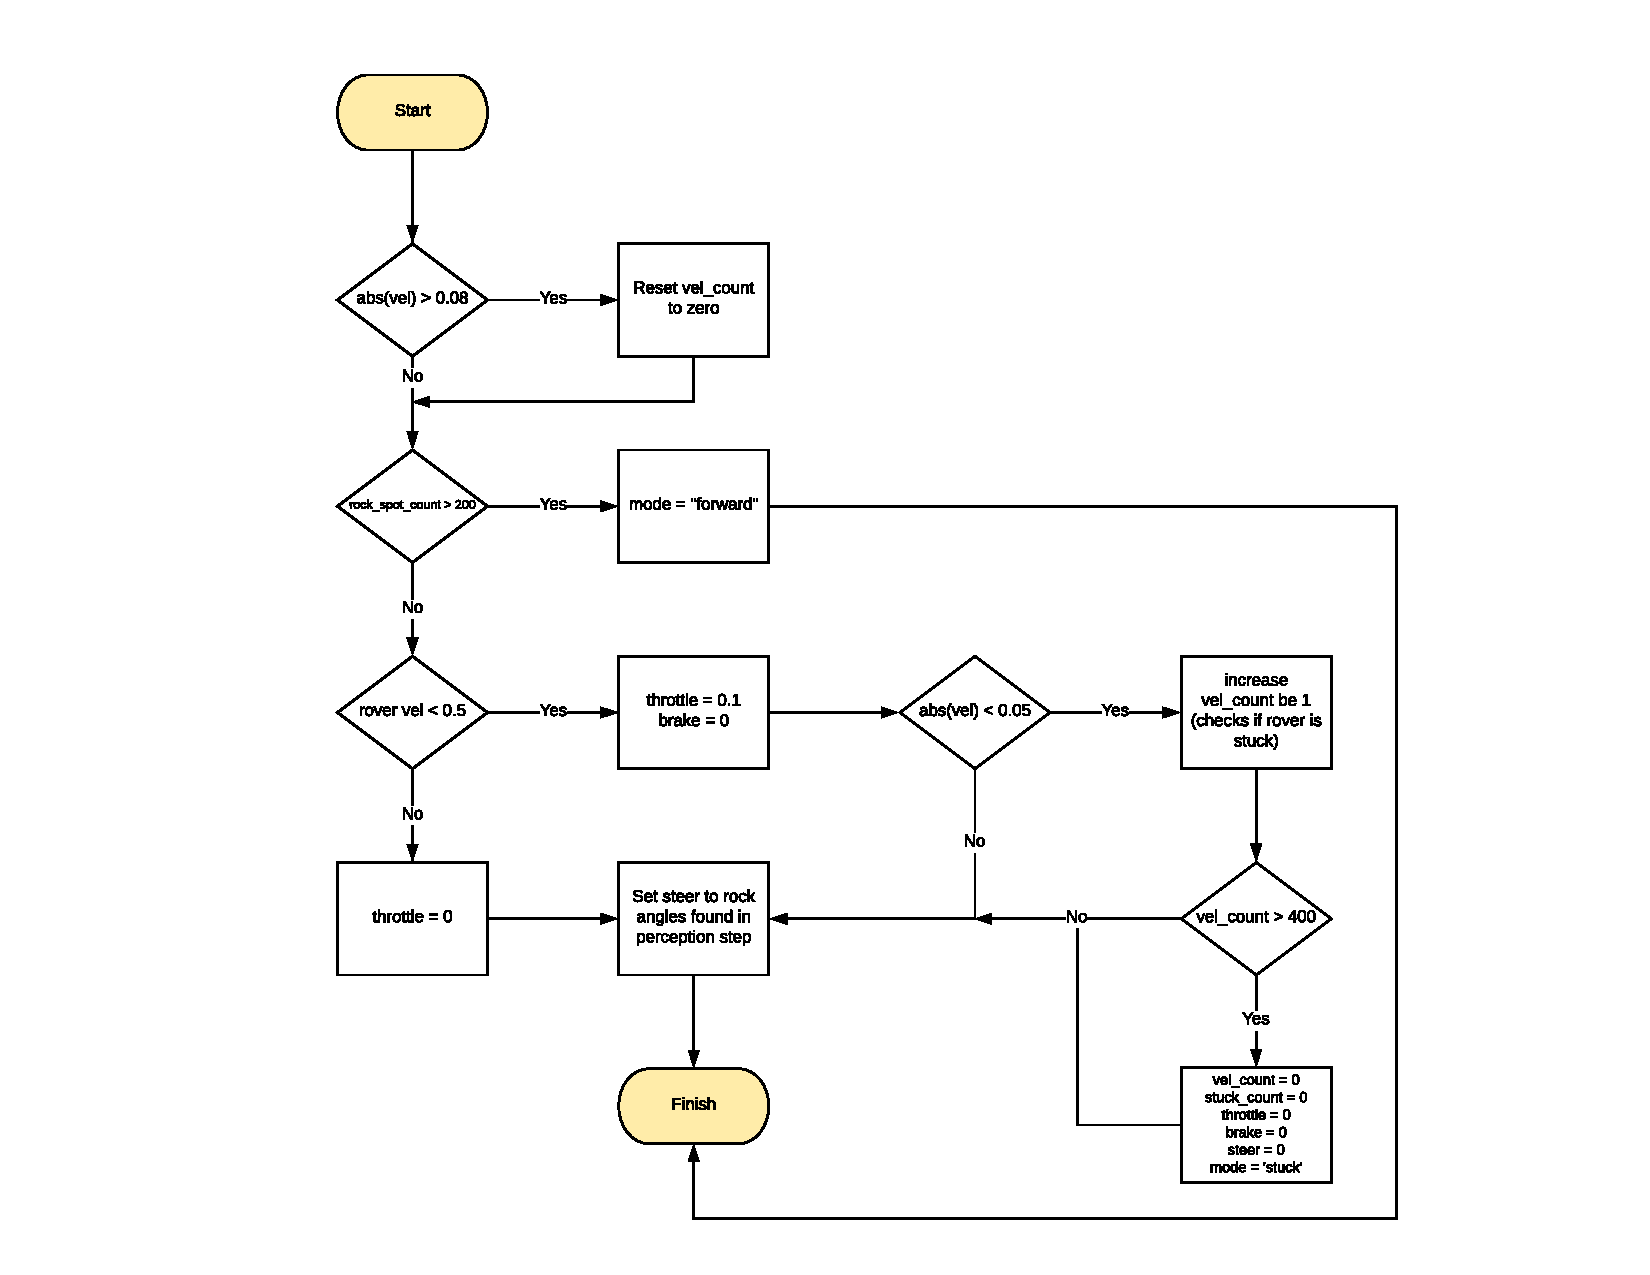
\includegraphics[scale=0.7]{rocking_flow}
\caption{Flow diagram showing the operation of the rover when it is in the rocking state of operation.}
\end{figure}

The stuck state code snippet can be seen in Listing 16, and the flow diagram explaining the logic behind the operation is shown in Figure 23. When the rover is in the stuck state, a counter is increased by one, and the throttle is set to -0.1, with the steering angle set to 0 so the rover will reverse away from the obstacle. The rover will persist in this mode until the counter reaches 300, at which time the rover will change states to the forward state.\\

\begin{figure}[h]\scriptsize
\begin{sexylisting}{Code snippet showing the operation of the rover in the stuck state}
# This is the Rover stuck mode - that is if the wheels are caught on the terrain        
        elif Rover.mode == 'stuck':
            Rover.stuck_count += 1 # Add a count to the hysteresis
            Rover.steer = 0
            Rover.throttle = -0.1 # This will reverse the rover with 0 steer angle
            Rover.brake = 0
            
            # This behaviour, once triggered only needs to occur for 300 processed frames
            # which is less than 10 seconds
            if Rover.stuck_count > 300:
                Rover.stuck_count = 0 # Reset the stuck counter
                Rover.steer = 0 # Reset the Rover steering
                Rover.mode = 'forward' # Hopefully the rover is unstuck
\end{sexylisting}
\end{figure}

\begin{figure}[h]
\hspace{-1.5cm}
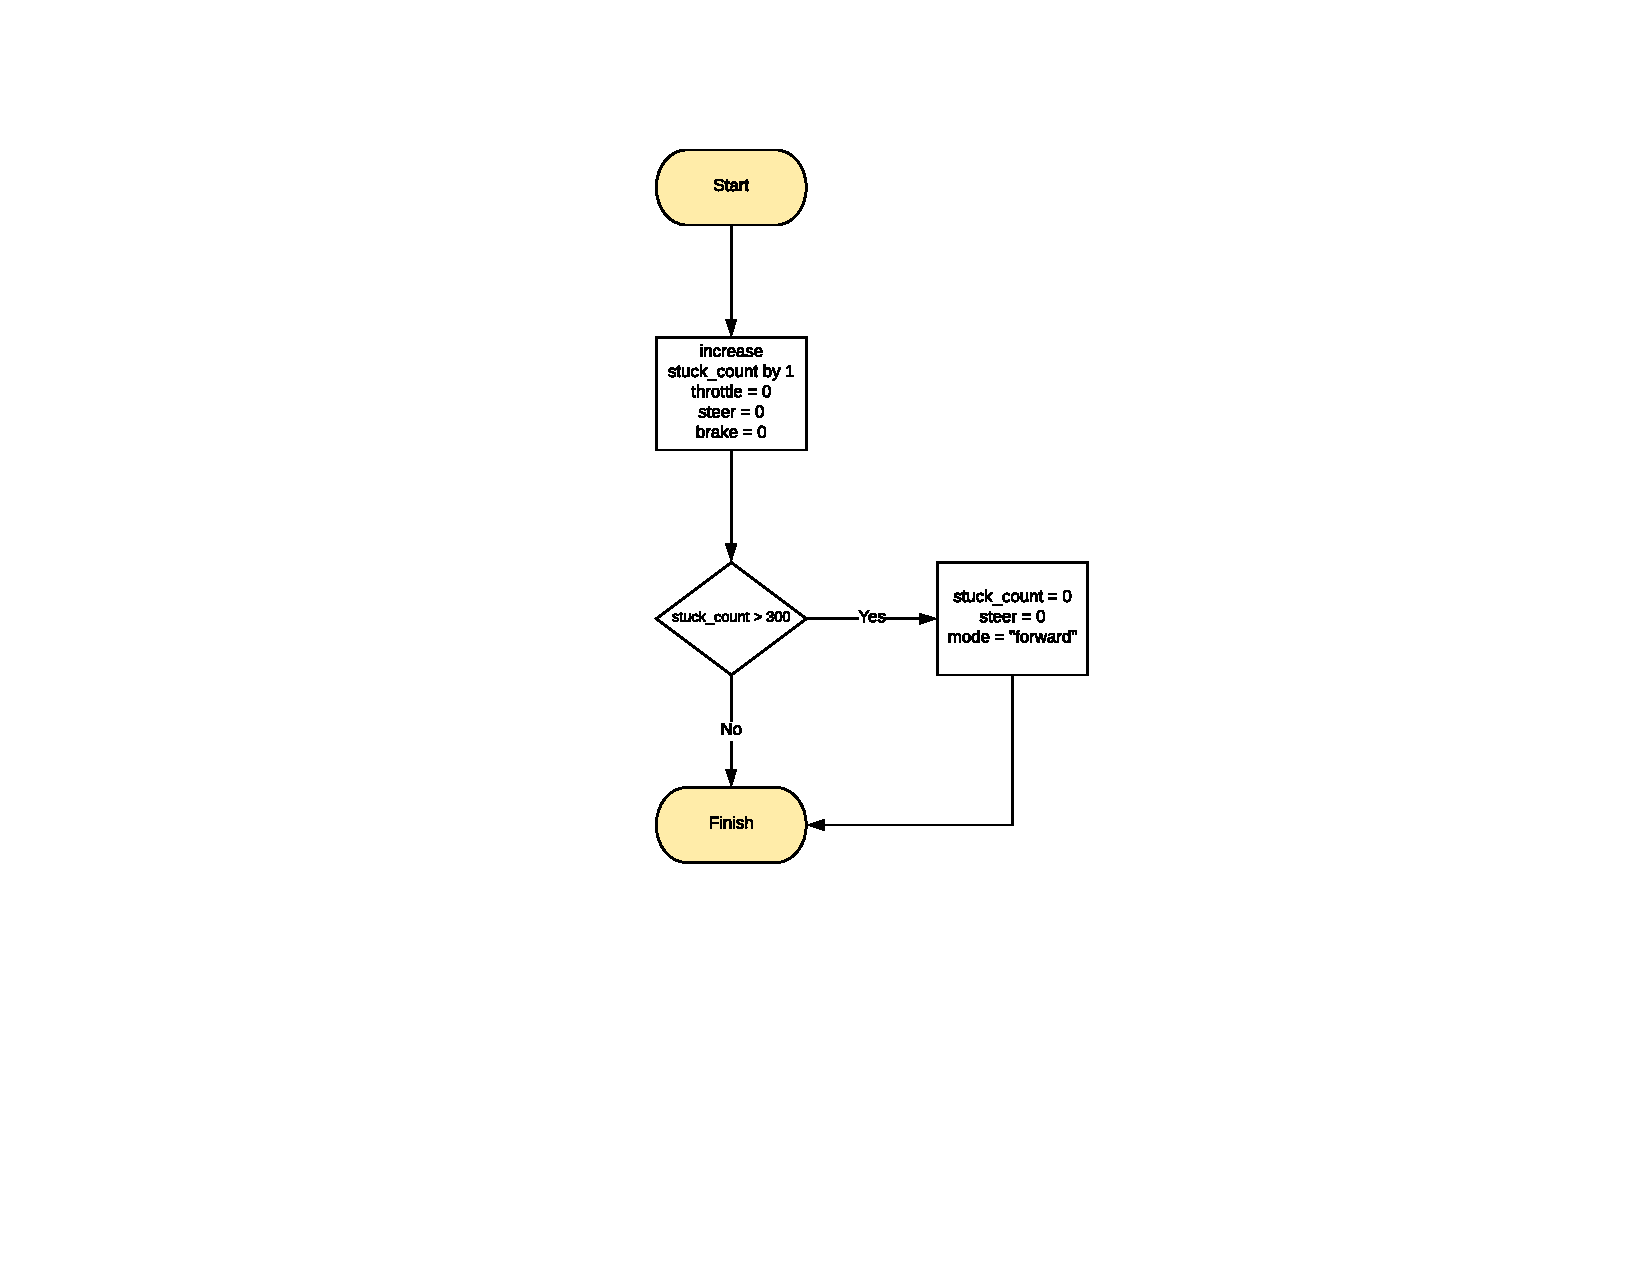
\includegraphics[scale=0.7]{stuck_flow}
\vspace{-3cm}
\caption{Flow diagram showing the operation of the rover when it is in the stuck state of operation.}
\end{figure}

\clearpage


Finally, the stop state code snippet can be seen in Listing 17, and the flow diagram explaining the logic behind the operation is shown in Figure 24. When in the stop state, the rover will first check if the velocity is greater than 0.2, in which case it will apply the brake to bring the rover to a rapid stop. The rover will then check the navigable terrain. If there is no navigable terrain, then the rover will turn counter clockwise on the spot, until sufficient navigable terrain is visible. At this point the rover will recommence in the forward state.

\begin{figure}[h]\scriptsize
\begin{sexylisting}{Code snippet showing the operation of the rover in the stop state}
# If we're already in "stop" mode then make different decisions
        elif Rover.mode == 'stop':
            # If we're in stop mode but still moving keep braking
            if Rover.vel > 0.2:
                Rover.throttle = 0
                Rover.brake = Rover.brake_set
                Rover.steer = 0
            # If we're not moving (vel < 0.2) then do something else
            elif Rover.vel <= 0.2:
                # Now we're stopped and we have vision data to see if there's a path forward
                if len(Rover.nav_angles) < Rover.go_forward:
                    Rover.throttle = 0
                    # Release the brake to allow turning
                    Rover.brake = 0
                    # Turn range is +/- 15 degrees, when stopped the next line
                    # will induce 4-wheel turning
                    Rover.steer = -15 # Could be more clever here about which way to turn
                # If we're stopped but see sufficient navigable terrain in front then go!
                if len(Rover.nav_angles) >= Rover.go_forward:
                    # Set throttle back to stored value
                    Rover.throttle = Rover.throttle_set
                    # Release the brake
                    Rover.brake = 0
                    # Set steer to mean angle
                    Rover.steer = np.clip(np.mean(Rover.nav_angles * 180/np.pi), -15, 15)
                    Rover.mode = 'forward'
\end{sexylisting}
\end{figure}

\begin{figure}
\hspace{-1.5cm}
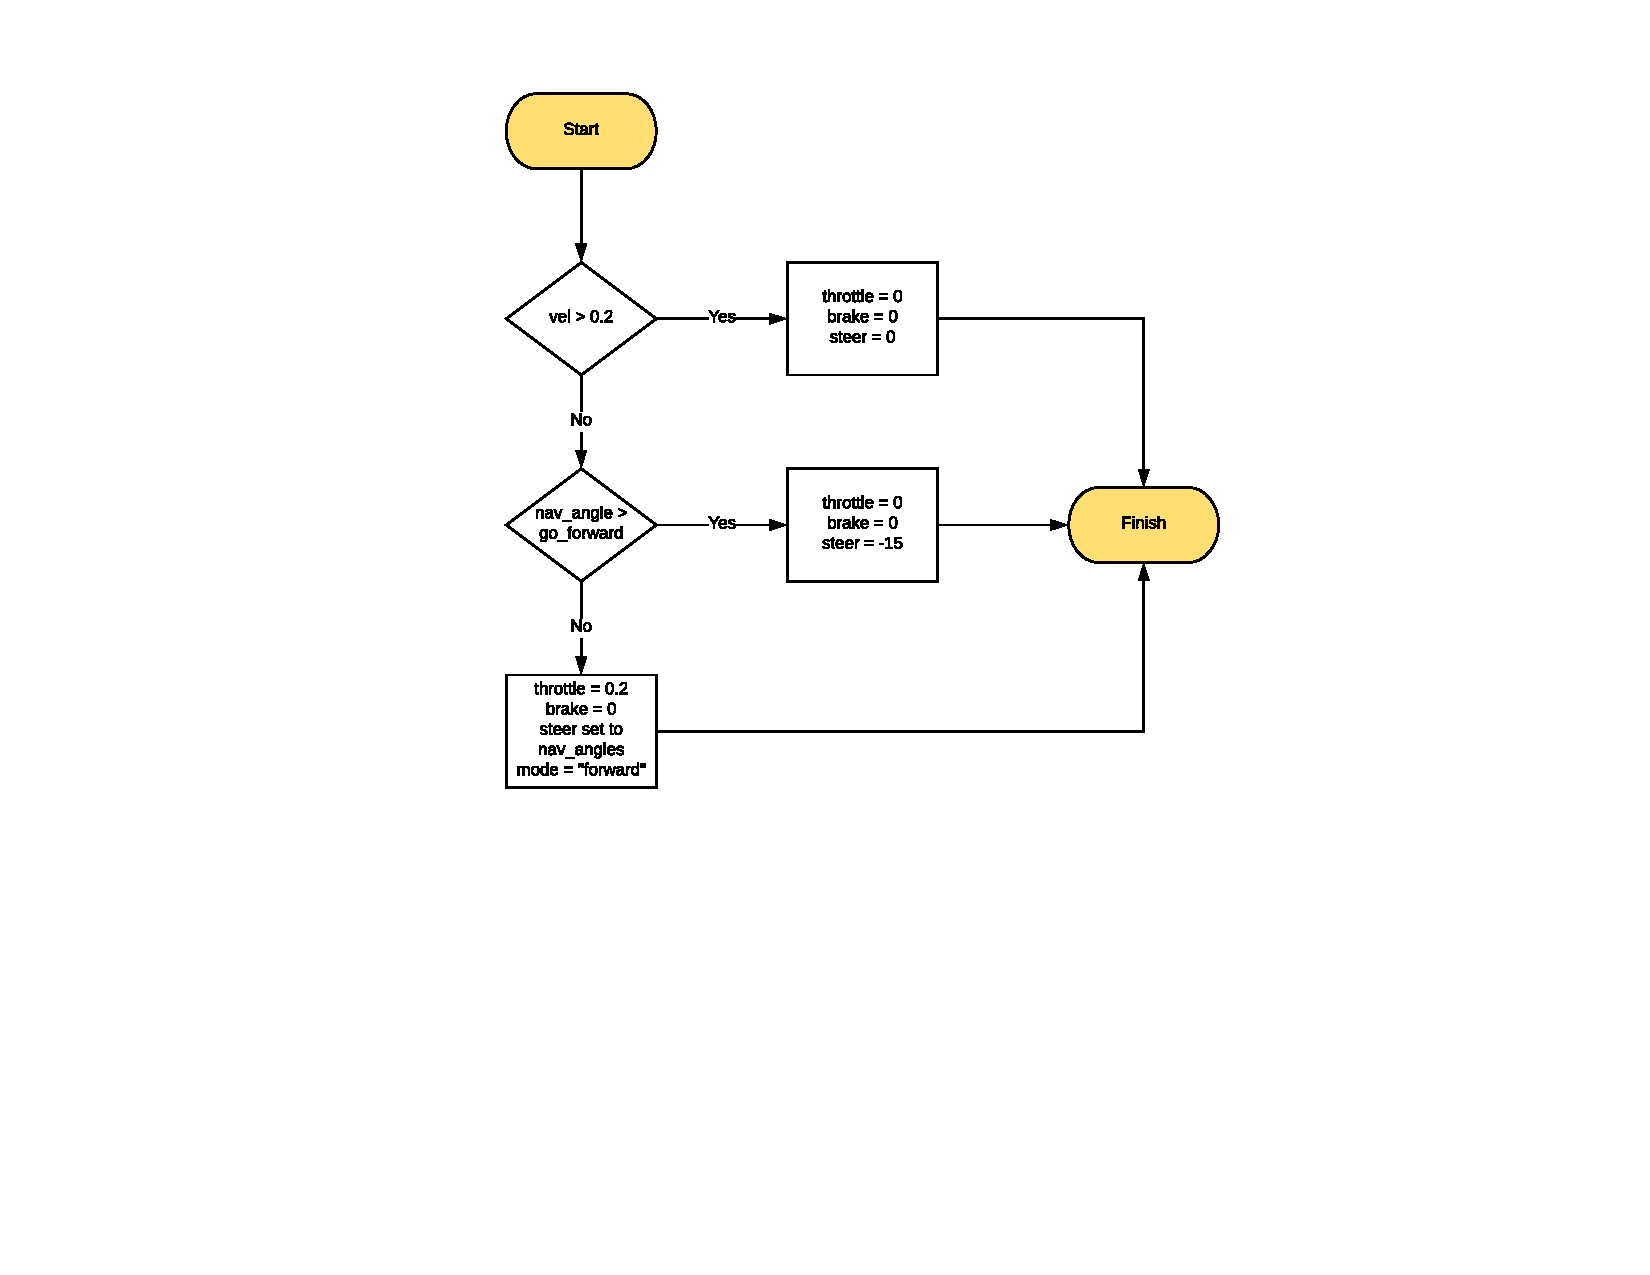
\includegraphics[scale=0.7]{stop_flow}
\caption{Flow diagram showing the operation of the rover when it is in the stuck state of operation.}
\end{figure}

%--------------------------------------------------------------------------
\section{Results \& Conclusion}

The code implementations seen in the perception step and the decision step allowed the rover to navigate the map in almost all circumstances. The full set of code implementations can be found at the following Github repository:

\begin{center}
	\url{https://github.com/skreynolds/RoboND-Rover-Project.git}
\end{center}

There were only a few minor instances where the rover would become stuck with no chance to recover. These minor situations would occur when the rover would have the undercarriage balanced on a rock providing no contact between the rover wheels and the ground, or places that the rover itself would become embedded into the obstacle. A video of the rover navigating successfully through the terrain can be seen at the following YouTube link:

\begin{center}
	\url{https://youtu.be/-hOlGIr9gxk}
\end{center}

The implementation was able to map well over the required 40\% of the map, and the fidelity of the mapping never fell below 80\% - most of the time it was above 90\%. Further, the rover was able to autonomously locate rock samples and pick them up in most instances.

\newpage

%--------------------------------------------------------------------------

\section{Further Enhancements}

Enhancements could be made by instructing the rover to return back to its original position when it has found all of the rock samples present in the map. This would require the rover to take note of the Cartesian coordinates at which it was positioned when the simulation started. Further, the number of samples collected would also need to be monitored. When the rover had collected 6 samples (this is the number of samples in each simulation), then the rover would switch to a newly created state which would see the rover return to its original position. Further, adjustments to the rover's forward state of navigation may help it to avoid areas which cause it to becomes irrecoverably stuck.

\newpage

\section{Appendix A}

\lstset{
	frame       = single,
	numbers     = left,
	showspaces  = false,
	showstringspaces    = false
}

\tiny
\lstinputlisting[style=Python]{./code/perception.py}

\newpage

\section{Appendix B}

\tiny
\lstinputlisting[style=Python]{./code/drive_rover.py}

\newpage

\section{Appendix C}

\tiny
\lstinputlisting[style=Python]{./code/decision.py}

\end{document}